\chapter{Server}

\section{Server features}

The server can be seen as an interface between the clients and the simulator.
All requests coming from the clients and that modify the tree are forwarded to
the simulator.\\

The server is multi-client but manages only one simulation at a time. When a
client connects, the server sends its status (file open, simulation running).\\

The server is autonomous because some simulations can take hours to days to
finnish. The idea is that the user can launch a simulation before leaving work
and then closes the client. He must be able to see the simulation running from
his home computer (if the computer on which the server is running is accessible
from the Internet).

%++++++++++++++++++++++++++++++++++++++++++++++++++++++++++++++++++++++++++++
%++++++++++++++++++++++++++++++++++++++++++++++++++++++++++++++++++++++++++++
%++++++++++++++++++++++++++++++++++++++++++++++++++++++++++++++++++++++++++++
%++++++++++++++++++++++++++++++++++++++++++++++++++++++++++++++++++++++++++++

\section{Encountered problems and their solution}

\subsection{Concurrent access protection}

A recurring problem with a multi-client server is the concurrent access. Here,
there may be an concurrent access when two clients try to modify the tree at
the same time or a client requesting the tree while it is being modified. This
can cause errors or, in the second case, an inconsistent tree.\\

To avoid this, when the server recieves a request:
\begin{itemize}
 \item it gets locked;
 \item it sends the request to \cf and waits for a answer from \cf;
 \item when \cf answers, if the resquest was well executed, the server
sends the modified tree to all clients (if there was an error, it is forwarded
to the client that sent the request);
 \item once the tree has been sent to all clients, the server gets unlocked.
\end{itemize}

When the server is locked, any new request for \cf is rejected until the server
is unlocked again.

%----------------------------------------------------------------------------
%----------------------------------------------------------------------------

\subsection{Thread and simulator}

A program is composed of tasks. For example, \inQuotes{\textit{Open a file}} is
a task. Only one task can be executed at a time. For some reasons, this program
may need to do more than one task at a time. To allow this, tasks are excecuted
in separated threads, exactly as if they were different programs, but with the
advantage that all threads coming from a program can use shared data very
easily. \\

A such program is \textit{multi-threaded}. A program is never multi-threaded by
default. It is up to the developer to decide which tasks can be run in a
separated thread. Because of the shared data, a concurrent access protection
may be necessary, but not only on data. This may be done on code portions.\\

When the simulation is running, the server would not accept neither new clients
connection nor requests to modify the tree until the simulation is done. This
would not be possible because the simulator is not multi-threaded. During the
simulation, the server waits for it to finish and can not do anything else. If
a client gets connected or sends a request, the server would not respond until
the simulation is finished.\\

\begin{figure}[H]
 \begin{center}
  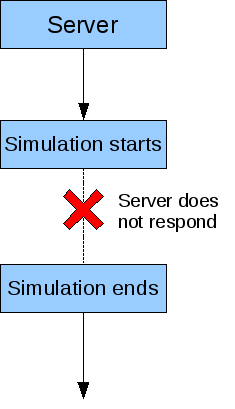
\includegraphics[width=0.25\textwidth]{images/serverWithoutThread}
 \end{center}
\caption{Simulation running on a server without a thread}
\end{figure}

To avoid this, the simulation is executed in a separated thread. The server
does not wait, can process client requests and is noticed when the simulation
is done.\\

\begin{figure}[H]
 \begin{center}
  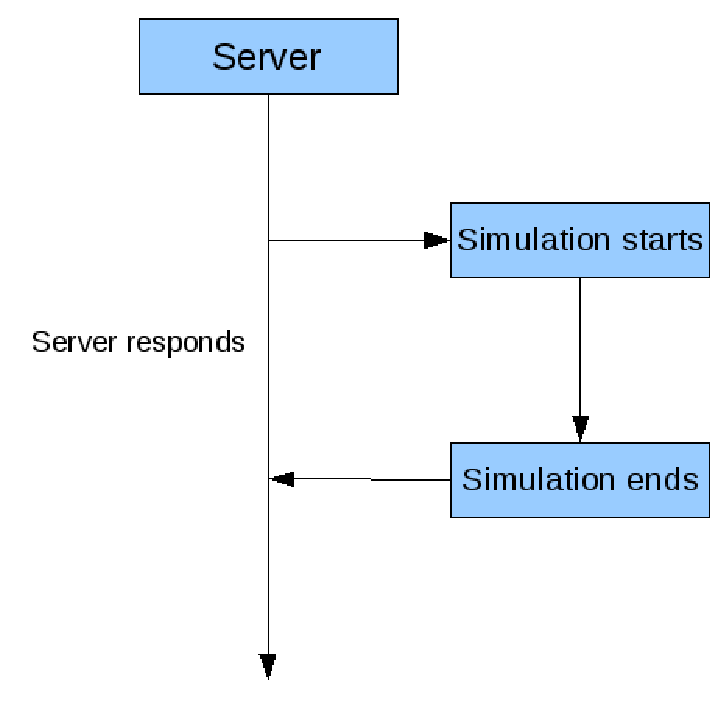
\includegraphics[width=0.5\textwidth]{images/serverWithThread}
 \end{center}
\caption{Simulation running on a server with a thread}
\end{figure}

%----------------------------------------------------------------------------
%----------------------------------------------------------------------------
